\documentclass{proc}

\usepackage{edbkps}
\usepackage{amsmath}
\usepackage{amssymb}
\usepackage{setspace}
\usepackage[utf8]{inputenc}
\usepackage{setspace}
\usepackage{subfig}
%%\usepackage[lined,boxed,commentsnumbered, linesnumbered]{algorithm2e}



\setcounter{secnumdepth}{2}
\setcounter{tocdepth}{0}
\let\footnote\savefootnote
\let\footnotetext\savefootnotetext
\let\footnoterule\savefootnoterule
\normallatexbib
\makeatletter
\renewcommand{\@ptsize}{0}
\makeatother

%%%%%
%% If you use a font encoding package, please enter it here, i.e.,
\usepackage{t1enc}


%%%%%
% Style for inserting .eps files and rotating illustrations or tables

% possible options for graphicx:
% [dvips], [xdvi], [dvipdf], [dvipsone], [dviwindo], [emtex], [dviwin],
% [pctexps],  [pctexwin],  [pctexhp],  [pctex32], [truetex], [tcidvi],
% [oztex], [textures]

\usepackage[dvips]{graphicx}
\usepackage[x11names, rgb]{xcolor}
\usepackage{tikz}
\usetikzlibrary{snakes,arrows,shapes}
\usepackage{amsmath}

%%%%%%%%%%%%%%%%%%%%%%%%%%%%%%%%%%%%%%%%%%%%%%%%%%%%%%%%%%%%%%%%%%%%%%%%%

\begin{document}


\articletitle[Decomposição Lagrangeana]
{Decomposição Lagrangeana}

\author{João C. Abreu\altaffilmark{1}}

\altaffiltext{1}{Universidade Federal de Minas Gerais, DCC, \\
Avenida Antônio Carlos 6627, Belo Horizonte, Brazil,\\
\email{joao.junior@dcc.ufmg.br}}

\anxx{João C. Abreu Jr.,Universidade Federal de Minas Gerais\,
Avenida Antônio Carlos 6627\, Belo Horizonte\, Brasil\,
\emailfont{joao.junior@dcc.ufmg.br}}

\begin{abstract}
Esse relatório apresenta a decomposição lagrangeana e o algoritmo do volume para resolver um problema proposto.

\end{abstract}

\begin{keywords}
\inx{Decomposição Lagrangeana}, \inx{Método do Volume}
\end{keywords}

\doublespacing

\section{Introdução}
\label{sec:intro}
O Problema composto pela função objetivo \eqref{eq:objetivoa} e as restrições \eqref{eq:arvore}-\eqref{eq:binaria},
onde as restrições \eqref{eq:arvore}-\eqref{eq:arvore2} formam uma árvore, e a restrição \eqref{eq:grau} representa
a quantidade máxima de arestas escolhidas incidentes a um nó $i \in V$,
\begin{align}
    & min \sum_{e \in E} c_ex_e \label{eq:objetivoa} \\
    & \text{Sujeito à:} \nonumber \\
    & \sum_{e \in E} =  n - 1 \label{eq:arvore} \\
    & t_i - t_j + |V|x_{ij} \le |V| - 1 \textrm{,} \forall (i,j) \in E \label{eq:arvore1} \\
    & 0 \le t_i \le |V| \textrm{,} \forall i \in V \label{eq:arvore2} \\
    & \sum_{e \in \delta(i)} x_e \le b_i \textrm{,} \forall i \in V \label{eq:grau} \\
    & x_e \in \{0, 1\} \label{eq:binaria}
\end{align}

Pode ser decomposto como:
\begin{align}
    & min \frac{1}{2}\sum_{e \in E} c_ez_e +  \frac{1}{2}\sum_{e \in E} c_ev_e\label{eq:objetivodecomposto}  \\
    & \text{Sujeito à:} \nonumber \\
    & z \in T \label{eq:arvored} \\
    & v \in M \label{eq:matchingd} \\
    & z = v \label{eq:ma} \\
    & (z,v) \in \{0,1\}^{2m} \label{eq:2m}
\end{align}
Associando multiplicadores de lagrange $\pi$ a restrição \eqref{eq:ma}, teremos o seguinte problema de lagrange a ser resolvido:
\begin{align}
    & \theta(\pi) = min \frac{1}{2}\sum_{e \in E} c_ez_e +  \frac{1}{2}\sum_{e \in E} c_ev_e + \sum_{e \in E} \pi(z_e - v_e) \label{eq:objetivodecomposto1}  \\
    & \text{Sujeito à:} \nonumber \\
    & z \in T \label{eq:arvored1} \\
    & v \in M \label{eq:matchingd1} \\
    & (z,v) \in \{0,1\}^{2m} \label{eq:2m1}
\end{align}

\section{Algoritmo}\label{sec:algoritmo} 
A figura \ref{AlgoritmoVolume} apresenta o algoritmo do volume revisado adaptado para o problema lagrangeano
$ \theta (\pi)$ retirado de \cite{Barahona91}. 
\begin{figure}
\centering
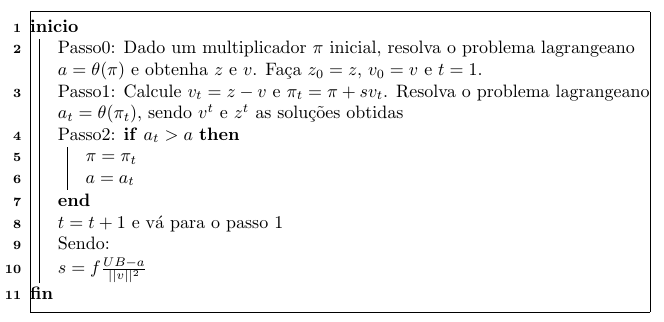
\includegraphics[width=4in]{AlgoritmoVolume.png}
\caption{Algoritmo do método do volume para o problema lagrangeano $ \theta (\pi)$}
\label{AlgoritmoVolume}
\end{figure}

\section{Experimentos Computacionais}\label{sec:experimentos} 
Os experimentos computacionais foram executados em uma máquina Intel Dual-Core de 2.81 GHz de clock e
2GB de memória RAM, rodando o sistema operacional Linux. O modelo matemático composto pela função objetivo \eqref{eq:objetivodecomposto} e
as restrições \eqref{eq:arvored}-\eqref{eq:2m} foi implementado
no Ilog CPLEX 12.5.1 e o algoritmo da seção \ref{sec:algoritmo} foi implementado
em Python 2.7, sendo que o otimizador utilizado para resolver o problema lagrangeano $\theta (\pi)$ presente nesse algoritmo foi o Ilog CPLEX 12.5.1.
As instâncias de testes utiizadas são denominadas ANDINST e foram propostas em \cite{Andrade06}.

No experimento desse trabalho foi comparado a performance do modelo matemático composto pela função objetivo \eqref{eq:objetivodecomposto} e
as restrições \eqref{eq:arvored}-\eqref{eq:2m} que será 
chamado aqui de $IP$, com o algoritmo proposto na seção \ref{sec:algoritmo}, que será chamado $Volume$.
O modelo $IP$ foi executado através do CPLEX com todos os parâmetros default. O modelo presente no algoritmo $Volume$
foi executado pelo CPLEX também com os valores default. O algoritmo $Volume$ foi executado com os parâmetros 
$f = 0.01$, com um número máximo de iterações igual a 500000. O modelo $IP$ e o algoritmo $Volume$ foram executados com um tempo de execução máximo de 7200 segundos. \\ 

A tabela \ref{table:resultados4e6} apresenta os resultados obtidos para o conjuntos de instância de testes. Nessa tabela a
coluna 1 mostra o nome da instância de teste, as colunas 2 e 3 são resultados referentes ao modelo $IP$ e as colunas
4,5 e 6 são resultados referentes ao algoritmo $Volume$. A coluna 2 apresenta o custo da solução obtido pela
modelo $IP$ e a coluna 3 apresenta o tempo consumido para encontrar essa solução. A coluna 4 apresenta o custo da solução 
obtido pelo algoritmo $Volume$, a coluna 5 traz o número de iterações do algoritmo
e a coluna 6 mostra o tempo consumido pelo algoritmo $Volume$.\\
Para todas as instâncias o CPLEX conseguiu encontrar soluções ótimas, conforme
pode ser observado pela coluna 2 da tabela \ref{table:resultados4e6}. O algoritmo
$Volume$ não conseguiu encontrar uma solução ótima ou próxima da ótima para nenhuma dessas instâncias, conforme
pode ser observado na coluna 4 da tabela \ref{table:resultados4e6}.

\begin{table}[htbp]
\begin{center}
  \begin{tabular}{|c|r|r|r|r|r|}
    \hline
      Instância & \multicolumn{2}{|c|}{$IP$} & \multicolumn{3}{|c|}{$Volume$}\\
                & Custo Solução    & Tempo(s)  & Custo Solução &Iterações & Tempo(s)      \\ \hline
        tb1ct100\_1 & 2722 & 4.01 & 2384.67 & 334 & 1340.68 \\ \hline
        tb1ct100\_2 & 2808 & 3.92 & 2408.08 & 275 & 1122.68 \\ \hline
        tb1ct100\_3 & 2958 & 4.00 & 2428.90 & 215 & 866.78 \\ \hline
        tb1ct200\_1 & 4353 & 58.20 & 3871.71 & 335 & 7200.00 \\ \hline
        tb1ct200\_2 & 4544 & 58.14 & 3851.35 & 219 & 7200.00 \\ \hline
        tb1ct200\_3 & 4741 & 58.29 & 4050.24 & 335 & 7200.00 \\ \hline
        tb1ct300\_1 & 5456 & 340.60 & 3572.75 & 43 & 7200.00 \\ \hline
        tb1ct300\_2 & 5713 & 338.77 & 3631.13 & 42 & 7200.00 \\ \hline
        tb1ct300\_3 & 5114 & 336.54 & 3222.22 & 42 & 7200.00 \\ \hline
        tb1ct400\_1 & 6232 & 1302.72 & 3426.63 & 13 & 7200.00 \\ \hline
        tb1ct400\_2 & 6458 & 1289.88 & 3450.62 & 13 & 7200.00 \\ \hline
        tb1ct400\_3 & 6148 & 1285.12 & 3244.81 & 13 & 7200.00 \\ \hline
        tb2ct500\_1 & 6725 & 3105.34 & 3450.36 & 5 & 7200.00 \\ \hline
        tb2ct500\_2 & 6702 & 3111.46 & 3310.76 & 5 & 7200.00 \\ \hline
        tb2ct500\_3 & 6928 & 3103.93 & 3367.94 & 5 & 7200.00 \\ \hline
  \end{tabular}
\caption{Comparação entre os custos da solução e tempos obtidos entre o modelo $IP$ e o algoritmo $Volume$}
\label{table:resultados4e6}
\end{center}
\end{table}
Todo código fonte produzido por esse trabalho pode ser obtido no endereço eletrônico: $https://github.com/joaojunior/decomposicao\_lagrangeana$


\bibliographystyle{plain}
%chapbblname{tp}  % The name of the .bbl file, what is normally the name of your .tex file.
\bibliography{tp} %\chapbibliography{gow}

\end{document}





% LocalWords:  comeca ij kj ji lll hardcoded eq ranqueamento recuperável RRSP
% LocalWords:  Recuperável Rent Minmax Regret Single Pair MSP SPP Cplex
